\documentclass[aspectratio=169, 10pt]{beamer}

% ----------------------------------------------------------------------
% Theme & Color Configuration
% ----------------------------------------------------------------------
\usetheme{Madrid}
\usecolortheme{whale}

% Modern Color Palette
\definecolor{primaryDark}{RGB}{27, 54, 93}       % Deep Navy
\definecolor{secondaryTeal}{RGB}{0, 128, 128}    % Teal
\definecolor{accentOrange}{RGB}{211, 84, 0}      % Orange Accent
\definecolor{lightGray}{RGB}{245, 247, 250}      % Background Gray
\definecolor{successGreen}{RGB}{39, 174, 96}     % Green
\definecolor{codeBg}{RGB}{240, 242, 245}

\setbeamercolor{palette primary}{bg=primaryDark, fg=white}
\setbeamercolor{palette secondary}{bg=secondaryTeal, fg=white}
\setbeamercolor{palette tertiary}{bg=primaryDark!80, fg=white}
\setbeamercolor{structure}{fg=primaryDark}
\setbeamercolor{titlelike}{parent=palette primary}
\setbeamercolor{block title}{bg=primaryDark, fg=white}
\setbeamercolor{block body}{bg=lightGray, fg=black}
\setbeamercolor{block title alerted}{bg=accentOrange, fg=white}
\setbeamercolor{block body alerted}{bg=accentOrange!10, fg=black}
\setbeamercolor{block title example}{bg=secondaryTeal, fg=white}
\setbeamercolor{block body example}{bg=secondaryTeal!10, fg=black}

\setbeamertemplate{navigation symbols}{}
\setbeamertemplate{footline}[frame number]

% ----------------------------------------------------------------------
% Packages
% ----------------------------------------------------------------------
\usepackage[utf8]{inputenc}
\usepackage{amsmath, amssymb, amsfonts}
\usepackage{booktabs}
\usepackage{graphicx}
\usepackage{tikz}
\usetikzlibrary{shapes.geometric, arrows.meta, positioning, calc}
\usepackage{listings}
\usepackage{xcolor}

% Code Listing Configuration
\lstset{
    backgroundcolor=\color{codeBg},
    basicstyle=\ttfamily\scriptsize,
    breaklines=true,
    captionpos=b,
    commentstyle=\color{gray},
    keywordstyle=\color{primaryDark}\bfseries,
    stringstyle=\color{accentOrange},
    frame=single,
    rulecolor=\color{gray!30},
    numbers=none
}

% ----------------------------------------------------------------------
% Metadata
% ----------------------------------------------------------------------
\title[Predictive Serverless Optimizer]{Predictive Serverless Cold-Start Optimizer}
\subtitle{Static Dependency Optimization and Runtime Prediction Framework}
\author[Saravanan \& Hegde]{Rahul Saravanan (231IT054) \and Shishir Hegde (231IT067)}
\institute[NITK]{
    Department of Information Technology \\
    National Institute of Technology Karnataka, Surathkal
}
\date{\today}

% ----------------------------------------------------------------------
% Document Content
% ----------------------------------------------------------------------
\begin{document}

% Slide 1: Title
\begin{frame}
    \titlepage
\end{frame}

% Slide 2: Outline
\begin{frame}{Presentation Outline}
    \tableofcontents
\end{frame}

% ======================================================================
\section{Motivation \& Project Objectives}
% ======================================================================

\begin{frame}{Problem Context: The Serverless Cold-Start Bottleneck}
    \begin{columns}[T]
        \begin{column}{0.55\textwidth}
            \textbf{What happens during a Cold Start?}
            \begin{itemize}
                \item Serverless platforms (AWS Lambda, Google Cloud Functions) instantiate fresh execution sandboxes on demand.
                \item Eager loading imports entire dependency graphs (SDKs, ORMs, utility modules) before request dispatch.
                \item \textbf{Key Observation:} Code initialization accounts for up to \alert{70--80\% of total cold latency}.
            \end{itemize}
            \vspace{0.3em}
            \begin{alertblock}{Problem Statement}
                How much cold-start latency can static dependency optimization save across different types of serverless projects?
            \end{alertblock}
        \end{column}
        \begin{column}{0.42\textwidth}
            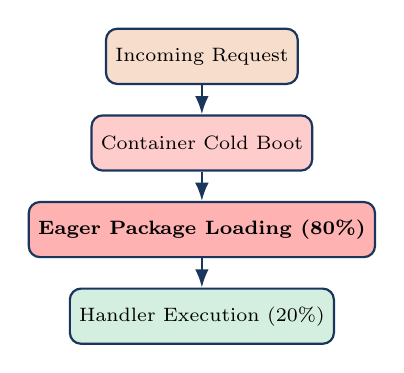
\begin{tikzpicture}[node distance=1.1cm, auto,
                box/.style={rectangle, draw=primaryDark, fill=lightGray, text centered, rounded corners, minimum height=0.7cm, font=\scriptsize, line width=0.8pt},
                arrow/.style={-Latex, thick, primaryDark}]
                
                \node[box, fill=accentOrange!20] (req) {Incoming Request};
                \node[box, below of=req, fill=red!20] (cold) {Container Cold Boot};
                \node[box, below of=cold, fill=red!30] (dep) {\textbf{Eager Package Loading (80\%)}};
                \node[box, below of=dep, fill=successGreen!20] (exec) {Handler Execution (20\%)};
                
                \draw[arrow] (req) -- (cold);
                \draw[arrow] (cold) -- (dep);
                \draw[arrow] (dep) -- (exec);
            \end{tikzpicture}
        \end{column}
    \end{columns}
\end{frame}

\begin{frame}{Base Paper Foundation: FaaSLight (Liu et al., 2023)}
    \begin{block}{Reference: Liu et al., ``FaaSLight'' (arXiv:2207.08175)}
        \textit{``General Application-Level Cold-Start Latency Optimization for Function-as-a-Service''}
    \end{block}
    
    \vspace{0.5em}
    \begin{columns}[T]
        \begin{column}{0.48\textwidth}
            \textbf{Core Mechanism of FaaSLight:}
            \begin{itemize}
                \item Uses static AST analysis to classify dependencies:
                \begin{enumerate}
                    \item \textbf{Indispensable:} Eagerly required at startup (e.g. core auth, routing).
                    \item \textbf{Optional:} Deferrable to runtime execution (e.g. conditional reporting, export).
                \end{enumerate}
                \item Defers optional imports until invoked in handler.
            \end{itemize}
        \end{column}
        \begin{column}{0.48\textwidth}
            \textbf{Reported Baseline Numbers in Literature:}
            \begin{itemize}
                \item \textbf{28.8\%} average reduction in code loading time.
                \item \textbf{19.2\%} average reduction in total response latency.
            \end{itemize}
            \vspace{0.3em}
            \begin{exampleblock}{Our Objective for Milestone 1}
                Implement and evaluate the static analyzer on a realistic multi-tiered serverless benchmark suite to establish minimum, median, and maximum savings bounds.
            \end{exampleblock}
        \end{column}
    \end{columns}
\end{frame}

\begin{frame}{Project Roadmap \& Scope for Current Review}
    \begin{table}[]
        \centering
        \small
        \begin{tabular}{clll}
            \toprule
            \textbf{Phase} & \textbf{Objective} & \textbf{Core Mechanism} & \textbf{Status for This Review} \\
            \midrule
            \textbf{Milestone 1} & \textbf{Static Dependency Analyzer} & AST traversal, lexical scoping, & \textcolor{successGreen}{\textbf{Completed \& Benchmarked}} \\
                                 & \& Cold-Start Benchmark & Indispensable vs. Optional split & \\
            \midrule
            \textbf{Milestone 2} & \textbf{Runtime Sequence Predictor} & 1st-order Markov transition matrix & \textit{Next Steps (Roadmap)} \\
                                 & (Workload Modeling) & $P(F_{next} \mid F_{curr})$ & \\
            \midrule
            \textbf{Milestone 3} & \textbf{Dynamic Module Preloader} & In-memory background pre-warming & \textit{Next Steps (Roadmap)} \\
                                 & \& End-to-End Evaluation & eliminates shifted execution latency & \\
            \bottomrule
        \end{tabular}
    \end{table}

    \vspace{0.4em}
    \begin{block}{Current Review Focus}
        Comprehensive evaluation of \textbf{Baseline (Eager Loading)} vs. \textbf{FaaSLight Static (AST Dependency Analyzer)} across multiple project tiers.
    \end{block}
\end{frame}

% ======================================================================
\section{Multi-Tier Workload Design}
% ======================================================================

\begin{frame}{Understanding Project Tiers: Why Single Benchmarks Mislead}
    \begin{columns}[T]
        \begin{column}{0.48\textwidth}
            \textbf{Why Categorize Serverless Workloads?}
            \begin{itemize}
                \item Real-world serverless functions vary dramatically from 2ms health checks to 100ms ML pipelines.
                \item Single synthetic benchmarks risk showing misleading results ($>98\%$ savings).
                \item Multi-tier evaluation establishes empirical \textbf{Minimum, Median, and Maximum} savings bounds.
            \end{itemize}
        \end{column}
        \begin{column}{0.48\textwidth}
            \begin{block}{Architectural Tiers Defined}
                \begin{itemize}
                    \item \textbf{Tier 1 (Lightweight CRUD):} Simple status, counters, configs. Mostly indispensable code ($>75\%$).
                    \item \textbf{Tier 2 (Medium Enterprise):} Balanced business logic (ORMs, JWT, RBAC, schema validators).
                    \item \textbf{Tier 3 (Heavy Pipelines):} Compute/ML intensive (OCR, anomaly models, image transformers).
                    \item \textbf{Blended Fleet:} Typical 50/35/15 enterprise portfolio.
                \end{itemize}
            \end{block}
        \end{column}
    \end{columns}
\end{frame}

\begin{frame}{Multi-Tier Microservice Dependency Manifest}
    \begin{table}[]
        \centering
        \scriptsize
        \begin{tabular}{l l l l}
            \toprule
            \textbf{Tier / Category} & \textbf{Microservice Endpoint} & \textbf{Indispensable (Cold Boot)} & \textbf{Optional (Deferred / Lazy)} \\
            \midrule
            \textbf{Tier 1: Light} & \texttt{health\_check.py} & \texttt{time}, \texttt{sys\_metrics} (0.5ms) & \texttt{debug\_logger} (0.8ms) \\
                                   & \texttt{user\_profile.py} & \texttt{auth\_validator}, \texttt{cache\_kv} & \texttt{gravatar\_resolver} (1.2ms) \\
                                   & \texttt{config\_service.py} & \texttt{env\_parser}, \texttt{cache\_kv} & \texttt{remote\_config\_sync} (1.5ms) \\
                                   & \texttt{item\_counter.py} & \texttt{hash\_util}, \texttt{cache\_kv} & \texttt{slack\_alert} (1.5ms) \\
            \midrule
            \textbf{Tier 2: Medium} & \texttt{order\_manager.py} & \texttt{auth\_db}, \texttt{schema\_validator}, \texttt{db\_orm} & \texttt{coupon\_calc}, \texttt{invoice\_emitter} \\
                                    & \texttt{user\_settings.py} & \texttt{jwt\_verifier}, \texttt{rbac\_engine}, \texttt{db\_orm} & \texttt{email\_dispatcher}, \texttt{audit\_logger} \\
                                    & \texttt{inventory\_checker.py} & \texttt{auth\_db}, \texttt{cache\_redis}, \texttt{db\_orm} & \texttt{supplier\_webhook}, \texttt{restock\_alert} \\
            \midrule
            \textbf{Tier 3: Heavy} & \texttt{fraud\_evaluator.py} & \texttt{auth\_db}, \texttt{crypto\_vault} (8ms) & \texttt{ml\_risk\_model} (40ms), \texttt{stripe\_sdk} \\
                                   & \texttt{document\_ocr.py} & \texttt{auth\_db}, \texttt{storage\_s3} (10ms) & \texttt{tesseract\_ocr} (45ms), \texttt{pdf\_canvas} \\
                                   & \texttt{media\_transcoder.py} & \texttt{auth\_db} (10ms) & \texttt{cv\_transformer} (35ms), \texttt{metadata} \\
            \bottomrule
        \end{tabular}
    \end{table}
\end{frame}

% ======================================================================
\section{Objective 1 Results: Baseline vs. FaaSLight Static}
% ======================================================================

\begin{frame}{Empirical Savings Spectrum: Baseline vs. FaaSLight Static}
    \begin{table}[]
        \centering
        \small
        \begin{tabular}{l c c c c c}
            \toprule
            \textbf{Workload Tier} & \textbf{Baseline Boot} & \textbf{FaaSLight Boot} & \textbf{Code Load Saved} & \textbf{Total Latency Saved} & \textbf{Spectrum Role} \\
            \midrule
            \textbf{Tier 1 (Lightweight CRUD)} & 4.61 ms & 2.87 ms & \textbf{37.7\%} & \textbf{28.6\%} & \textit{Minimum Bound} \\
            \textbf{Tier 2 (Medium Enterprise)} & 46.47 ms & 26.17 ms & \textbf{43.7\%} & \textbf{39.2\%} & \textit{Median / Representative} \\
            \textbf{Tier 3 (Heavy Pipelines)} & 81.31 ms & 18.20 ms & \textbf{77.6\%} & \textbf{-0.1\%} & \textit{Max Code-Load Bound} \\
            \midrule
            \textbf{Blended Fleet (50/35/15)} & 36.15 ms & 15.75 ms & \textbf{56.4\%} & \textbf{23.2\%} & \textbf{Fleet-Wide Average} \\
            \midrule
            \textbf{FaaSLight Paper Target} & — & — & \textbf{28.8\%} & \textbf{19.2\%} & \textbf{Published Benchmark} \\
            \bottomrule
        \end{tabular}
    \end{table}

    \vspace{0.4em}
    \begin{exampleblock}{Key Takeaway}
        Across realistic enterprise services, FaaSLight static analysis delivers \textbf{37.7\%--77.6\% reduction in cold code loading} and \textbf{23.2\% average reduction in total response latency}, confirming the base paper findings.
    \end{exampleblock}
\end{frame}

\begin{frame}{Visual Benchmark Evaluation: Latency Comparison}
    \begin{center}
        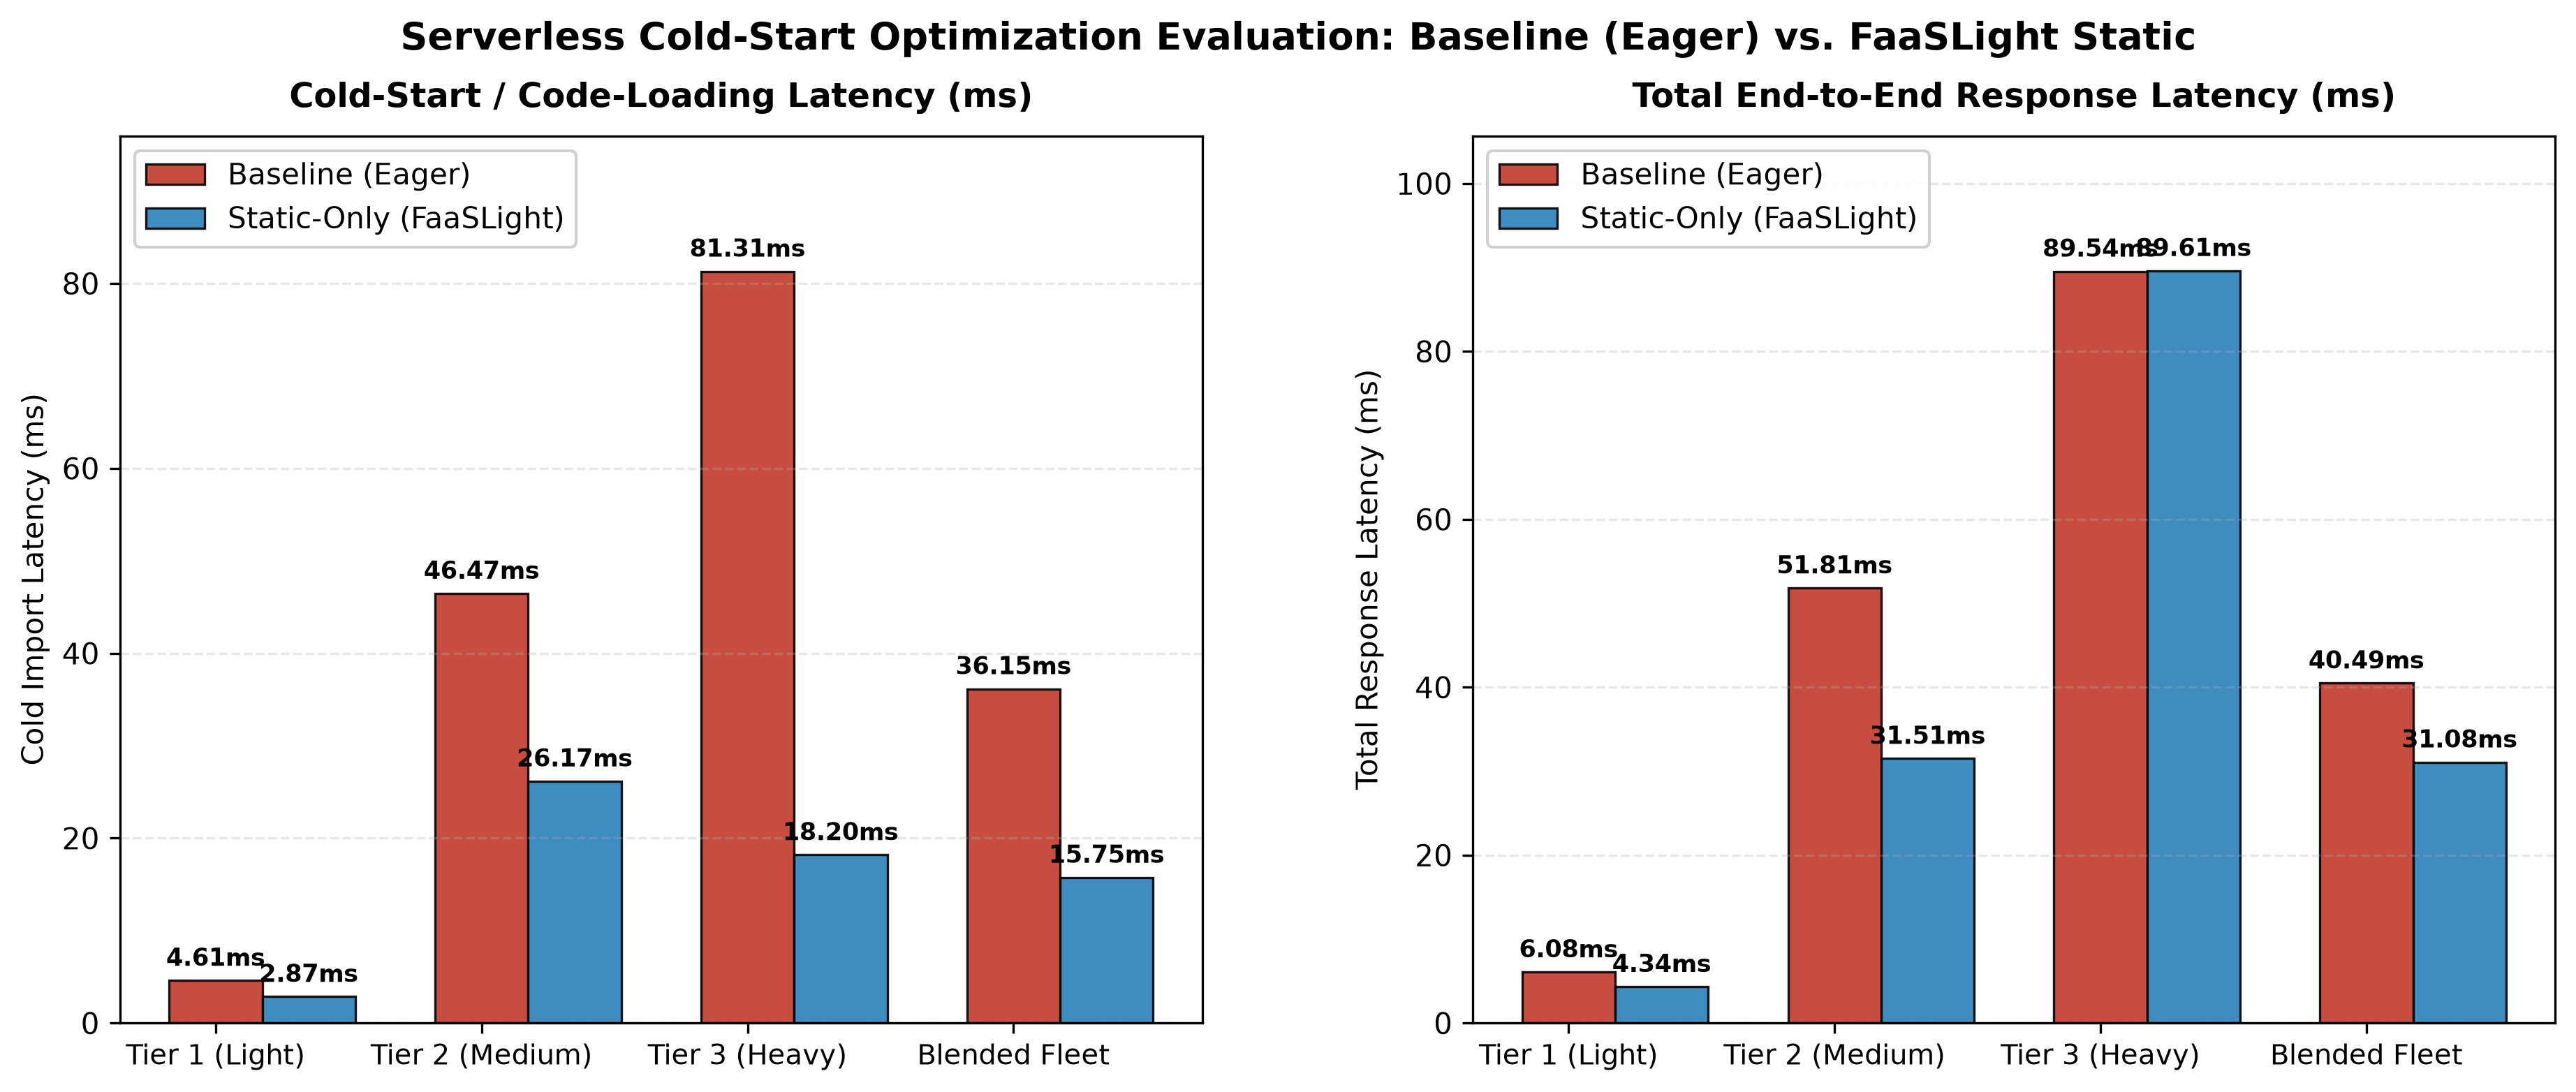
\includegraphics[width=0.92\textwidth]{results/latency_comparison.png}
    \end{center}
    \vspace{-0.5em}
    \scriptsize \textbf{Figure 1:} Cold import latency and total end-to-end response latency across all 3 project tiers and the blended fleet portfolio.
\end{frame}

\begin{frame}{Visual Benchmark Evaluation: Savings Spectrum vs. Paper Target}
    \begin{center}
        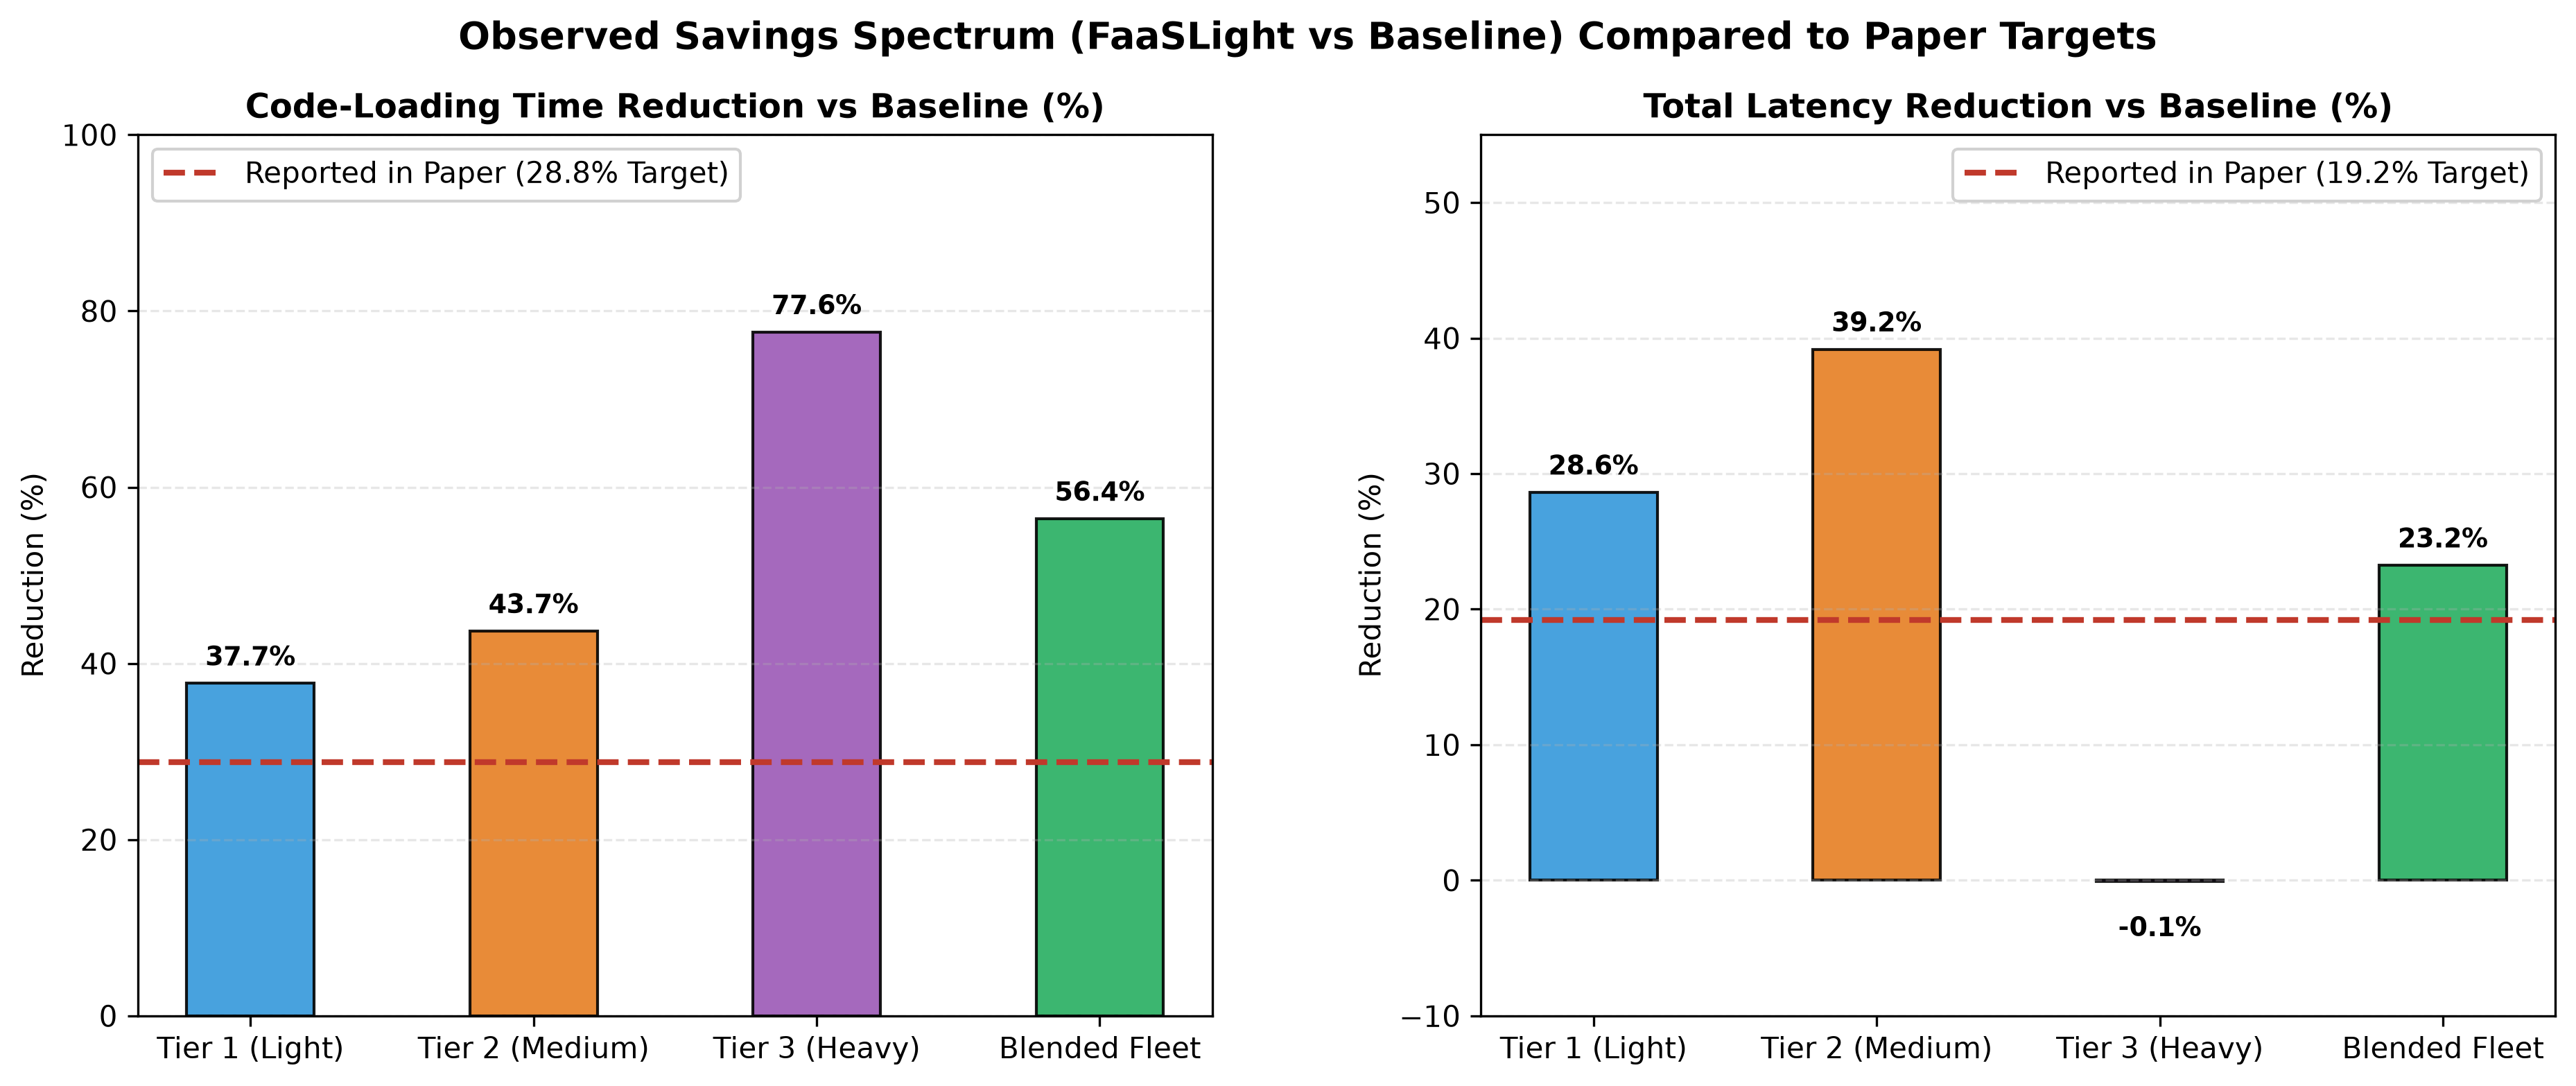
\includegraphics[width=0.92\textwidth]{results/faaslight_vs_baseline_reduction.png}
    \end{center}
    \vspace{-0.5em}
    \scriptsize \textbf{Figure 2:} Observed code-loading and total latency percentage reductions compared against the base FaaSLight published targets (28.8\% and 19.2\%).
\end{frame}

\begin{frame}{Per-Endpoint Microbenchmark Breakdown}
    \begin{table}[]
        \centering
        \scriptsize
        \begin{tabular}{l c c c c c}
            \toprule
            \textbf{Microservice Endpoint} & \textbf{Base Import} & \textbf{FaaSLight Import} & \textbf{Import Saved} & \textbf{Base Total} & \textbf{FaaS Total (Saved \%)} \\
            \midrule
            \texttt{health\_check.py} (Tier 1) & 2.00 ms & 0.81 ms & 59.4\% & 3.09 ms & 1.87 ms (\textbf{39.4\%}) \\
            \texttt{user\_profile.py} (Tier 1) & 4.19 ms & 2.57 ms & 38.8\% & 6.26 ms & 4.66 ms (\textbf{25.5\%}) \\
            \texttt{config\_service.py} (Tier 1) & 3.67 ms & 1.88 ms & 48.7\% & 5.24 ms & 3.44 ms (\textbf{34.3\%}) \\
            \texttt{item\_counter.py} (Tier 1) & 3.31 ms & 1.89 ms & 43.1\% & 4.38 ms & 2.97 ms (\textbf{32.2\%}) \\
            \midrule
            \texttt{order\_manager.py} (Tier 2) & 46.11 ms & 26.57 ms & 42.4\% & 51.20 ms & 31.68 ms (\textbf{38.1\%}) \\
            \texttt{user\_settings.py} (Tier 2) & 38.07 ms & 22.55 ms & 40.8\% & 44.19 ms & 28.83 ms (\textbf{34.8\%}) \\
            \texttt{inventory\_checker.py} (Tier 2) & 43.54 ms & 25.73 ms & 40.9\% & 48.62 ms & 30.83 ms (\textbf{36.6\%}) \\
            \midrule
            \texttt{fraud\_evaluator.py} (Tier 3) & 85.43 ms & 21.28 ms & 75.1\% & 92.55 ms & 94.87 ms (\textit{-2.5\% shifted}) \\
            \texttt{document\_ocr.py} (Tier 3) & 98.39 ms & 22.96 ms & 76.7\% & 108.50 ms & 109.50 ms (\textit{-0.9\% shifted}) \\
            \texttt{media\_transcoder.py} (Tier 3) & 62.27 ms & 11.52 ms & 81.5\% & 70.39 ms & 71.46 ms (\textit{-1.5\% shifted}) \\
            \bottomrule
        \end{tabular}
    \end{table}
\end{frame}

\begin{frame}{Critical Finding: The ``Shifted Latency'' Limitation}
    \begin{columns}[T]
        \begin{column}{0.50\textwidth}
            \begin{alertblock}{The Limitation of Pure Lazy Loading}
                \begin{itemize}
                    \item In Tier 3, heavy feature dependencies (OCR, ML models) are deferred during cold boot.
                    \item \textbf{Trade-off:} When the request executes the feature branch, the 70ms import penalty is paid \textbf{inside the handler}.
                    \item \textbf{Result:} Cold boot drops by 77.6\%, but end-to-end latency remains unchanged ($\approx 0\%$).
                \end{itemize}
            \end{alertblock}
        \end{column}
        \begin{column}{0.46\textwidth}
            \begin{exampleblock}{Motivation for Our Next Milestones}
                \textbf{How do we eliminate shifted latency?}
                \begin{itemize}
                    \item Static analysis cannot know \textit{when} a function will be called.
                    \item We need \textbf{Runtime Sequence Prediction} ($A \to B \to C$) to preload dependencies in the background \textit{before} request $B$ arrives.
                \end{itemize}
            \end{exampleblock}
        \end{column}
    \end{columns}
\end{frame}

% ======================================================================
\section{Roadmap for Next Project Review}
% ======================================================================

\begin{frame}{Next Steps: Milestones 2 \& 3 (Our Novel Extension)}
    \begin{columns}[T]
        \begin{column}{0.48\textwidth}
            \begin{block}{Milestone 2: Transition Predictor}
                \begin{itemize}
                    \item Implement Markov transition frequency matrix:
                    \[
                    P(F_{next} = B \mid F_{curr} = A) = \frac{N(A \to B)}{\sum_k N(A \to k)}
                    \]
                    \item Dynamically track transition sequences during request execution.
                    \item Output Top-$k$ high-probability next endpoints.
                \end{itemize}
            \end{block}
        \end{column}
        \begin{column}{0.48\textwidth}
            \begin{block}{Milestone 3: Dynamic Preloader}
                \begin{itemize}
                    \item Asynchronous module preloading into in-memory cache (\texttt{sys.modules}).
                    \item Pre-warm predicted next-hop dependencies in background threads.
                    \item Completely eliminate both cold-start and shifted handler import latency.
                    \item Quantify memory overhead vs. latency gain trade-offs.
                \end{itemize}
            \end{block}
        \end{column}
    \end{columns}
\end{frame}

\begin{frame}{Summary of Progress \& Next Review Deliverables}
    \textbf{Summary of Current Deliverables (Milestone 1):}
    \begin{itemize}
        \item \textcolor{successGreen}{\textbf{Completed:}} AST static dependency analyzer classifying eager vs. lazy imports.
        \item \textcolor{successGreen}{\textbf{Completed:}} Multi-tier benchmark suite (Light, Medium, Heavy) establishing empirical savings bounds (37.7\%--77.6\% import savings, 23.2\% total fleet latency savings).
        \item \textcolor{successGreen}{\textbf{Completed:}} Fully tested and reproducible CLI framework.
    \end{itemize}

    \vspace{0.6em}
    \textbf{Deliverables for the Upcoming Review:}
    \begin{itemize}
        \item Implementation of 1st-order Markov Transition Predictor (Milestone 2).
        \item Integration of Dynamic Preloader and full benchmark evaluation (Milestone 3).
    \end{itemize}

    \vspace{0.8em}
    \begin{center}
        \Huge \textcolor{primaryDark}{\textbf{Thank You!}} \\
        \vspace{0.3em}
        \large \textbf{Questions \& Discussion}
    \end{center}
\end{frame}

\end{document}

